


\chapter{Quotient Space and Simplicial Complex}

Motivation. Just like product space and disjoint union, we give another way to construct new topological spaces from some old ones. This new way of construction is by gluing some special pieces from old topological spaces together.

Idea. Let \(X = \left\lbrack  {0,1}\right\rbrack   \times  \left\lbrack  {0,1}\right\rbrack\) (just like a paper on a plane), we want to glue the leftmost edge with the rightmost edge to form a cylinder \({Y}_{1}\) , as shown below:

\begin{center}
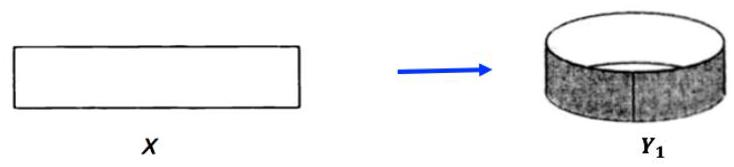
\includegraphics[max width=0.6\textwidth]{images/bo_d2bcsrref24c73avs720_60_452_764_734_167_0.jpg}
\end{center}
\hspace*{3em} 

If we give a half-twist to the strip before glue the ends together, we will get the Moebius stripe \({Y}_{2}\) shown below:

\begin{center}
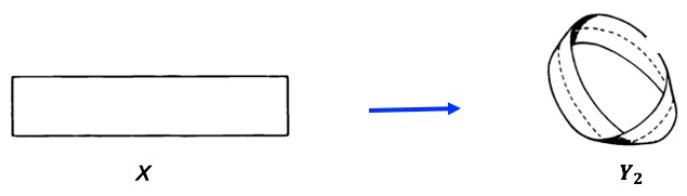
\includegraphics[max width=0.5\textwidth]{images/bo_d2bcsrref24c73avs720_60_448_1175_687_196_0.jpg}
\end{center}
\hspace*{3em} 

Interestingly, the first topology \({Y}_{1}\) has two sides, while the second has only one side.

\section*{5.6.2.1. Equivalence Relations and partitions}

Definition 5.7 [Equivalence Relation] The equivalence relation on a set \(X\) is a relation \~ such that

1. (Reflexive): \(x \sim  x,\forall x \in  X\)

2. (Symmetric): \(x \sim  y\) implies \(y \sim  x\)

3. (Transitive): \(x \sim  y\) and \(y \sim  z\) implies \(x \sim  z\) .

5.8 1. Let \(X = V\) be a vector space, and \(W \leq  V\) be a vector subspace. Define \({\mathbf{v}}_{1} \sim  {\mathbf{v}}_{2}\) if \({\mathbf{v}}_{1} - {\mathbf{v}}_{2} \in  W\) .

(The well-definedness is left as exercise).

2. (Mobius Stripe): Let \(X = \left\lbrack  {0,1}\right\rbrack   \times  \left\lbrack  {0,1}\right\rbrack\) . We define \(\left( {{x}_{1},{y}_{1}}\right)  \sim  \left( {{x}_{2},{y}_{2}}\right)\) if

\begin{itemize}
\item \({x}_{1} = {x}_{2},{y}_{1} = {y}_{2}\) ; (e.g., \(\left( {{0.5},{0.6}}\right)  \sim  \left( {{0.5},{0.6}}\right)\) ) or
\end{itemize}

\begin{itemize}
\item \({x}_{1} = 0,{x}_{2} = 1\) , and \({y}_{1} = 1 - {y}_{2}\) (e.g., \(\left( {0,1/4}\right)  \sim  \left( {1,3/4}\right)\) )
\end{itemize}

\begin{itemize}
\item \({x}_{1} = 1,{x}_{2} = 0\) , and \({y}_{1} = 1 - {y}_{2}\) (e.g., \(\left( {1,3/4}\right)  \sim  \left( {0,1/4}\right)\) )
\end{itemize}

Definition 5.8 [Partition] Let \(X\) be a nonempty set. A partition \(\mathcal{P} = \left\{  {{p}_{i} \mid  i \in  I}\right\}\) of \(X\) is a collection of subsets such that

1. \({P}_{i} \subseteq  X\) is non-empty

2. \({P}_{i} \cap  {P}_{j} = \varnothing\) if \(i \neq  j\)

3. \(\mathop{\bigcup }\limits_{{i \in  I}}{P}_{i} = X\)

R Given a partition \(\mathcal{P} = \left\{  {{p}_{i} \mid  i \in  I}\right\}\) , we can define an equivalence relation \(\sim\) on \(X\) by setting

\[
x \sim  y\;\text{ whenever }x,y \in  {p}_{i}\text{ , for some }i \in  I
\]

For example, if \(X = \left\lbrack  {0,1}\right\rbrack   \times  \left\lbrack  {0,1}\right\rbrack\) , then

\[
X = \{ \left( {x,y}\right) {\} }_{x \in  \left( {0,1}\right) ,y \in  \left\lbrack  {0,1}\right\rbrack  } \cup  \{ \left( {1,y}\right) ,\left( {0,1 - y}\right) {\} }_{y \in  \left\lbrack  {0,1}\right\rbrack  }
\]

gives a partition on \(X\) . This gives the same equivalence relation as in part (2) in example (5.8).

Conversely, given an equivalence relation \(\sim\) , we could form a corresponding partition of \(X\) . This kind of partition is called the equivalence class:

Definition 5.9 [Equivalence Class] Let \(X\) be a set with equivalence relation \(\sim\) . The equivalence class of an element \(x \in  X\) is

\[
\left\lbrack  x\right\rbrack   \mathrel{\text{ := }} \{ y \in  X \mid  x \sim  y\} .
\]

Proposition 5.8 The collection of all \(\left\lbrack  x\right\rbrack\) in \(X/ \sim\) gives a partition on \(X\) .

Consider the equivalence class defined in part (1) in example (5.8). The equivalence class has the form

\[
\left\lbrack  \mathbf{v}\right\rbrack   = \{ \mathbf{u} \in  V \mid  \mathbf{v} - \mathbf{u} \in  W\}  \mathrel{\text{ := }} \mathbf{v} + W.
\]

Therefore, the equivalence class is a generalization of the coset in linear algebra. Similarly, we define the set of generalized cosets as quotient space.

Definition 5.10 The collection of all equivalence classes is called the quotient space, denoted as \(X/ \sim\) , i.e.,

\[
X/ \sim   = \{ \left\lbrack  x\right\rbrack   \mid  x \in  X\} .
\]

9 1. Consider part (1) in example (5.8) again. The quotient space \(V/ \sim\) reduces to the \(V/W\) in linear algebra:

\[
V/ \sim   = \{ \left\lbrack  \mathbf{v}\right\rbrack   \mid  \mathbf{v} \in  V\}  = \{ \mathbf{v} + W \mid  \mathbf{v} \in  V\}  = V/W.
\]

2. Consider part (2) in example (5.8) again. Then \(X/ \sim\) essentially forms the Mobius band, e.g.,

\[
\left\lbrack  \left( {1/2,1/2}\right) \right\rbrack   = \{ x \mid  \left( {1/2,1/2}\right)  \sim  x\}  = \{ \left( {1/2,1/2}\right) \}
\]

\[
\left\lbrack  \left( {1,3/4}\right) \right\rbrack   = \{ x \mid  x \sim  \left( {1,3/4}\right) \}  = \{ \left( {1,3/4}\right) ,\left( {0,1/4}\right) \}
\]

\begin{itemize}
\item Example 5.10 Consider \(X = \left\lbrack  {0,1}\right\rbrack   \sqcup  \left\lbrack  {0,1}\right\rbrack\) , i.e.,
\end{itemize}

\[
X = \left( {\left\lbrack  {0,1}\right\rbrack  \times \{ 0\} }\right)  \cup  \left( {\left\lbrack  {0,1}\right\rbrack  \times \{ 1\} }\right)
\]

Take a partition on \(X\) by

\[
\{ \left( {a,0}\right) {\} }_{0 \leq  a < 1} \cup  \{ \left( {b,1}\right) {\} }_{0 < b \leq  1} \cup  \{ \left( {1,0}\right) ,\left( {0,1}\right) \}
\]

As a result, the corresponding quotient space is plotted below:

\begin{center}
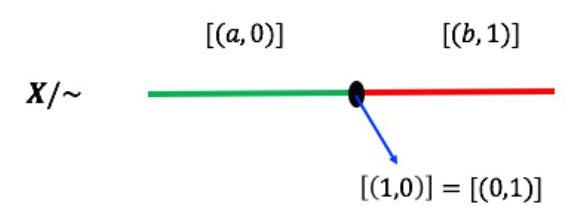
\includegraphics[max width=0.4\textwidth]{images/bo_d2bcsrref24c73avs720_63_632_857_565_216_0.jpg}
\end{center}
\hspace*{3em} 

\begin{itemize}
\item Example 5.11 Comes from \(X = \left\lbrack  {0,1}\right\rbrack   \times  \left\lbrack  {0,1}\right\rbrack\) with partition
\end{itemize}

\[
\{ \left( {a,b}\right) {\} }_{0 < a < 1;0 < b < 1} \cup  \{ \left( {x,0}\right) ,\left( {x,1}\right) {\} }_{0 \leq  x \leq  1} \cup  \{ \left( {0,y}\right) ,\left( {1,y}\right) {\} }_{0 < y < 1}
\]

The corresponding quotient space is plotted below:
\begin{center}
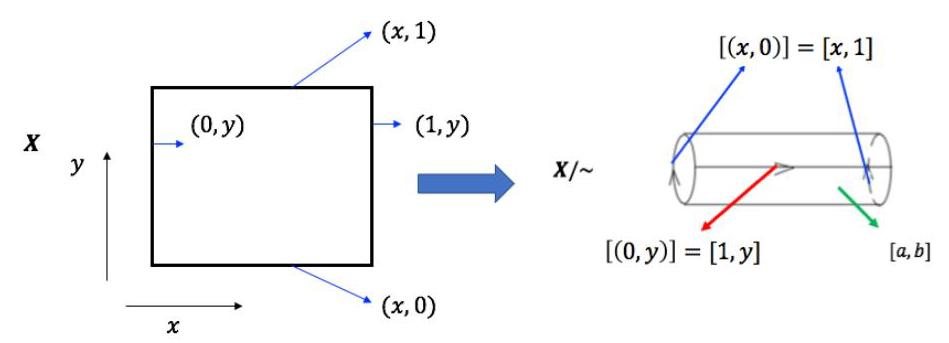
\includegraphics[max width=0.8\textwidth]{images/bo_d2bcsrref24c73avs720_63_491_1596_949_343_0.jpg}
\end{center}
\hspace*{3em} 

Proposition 5.9 Let(X, T)be topological space, with the equivalence relation. Define the canonical projection map

\[
p : \;X \rightarrow  X/ \sim
\]

\[
\text{ with }x \mapsto  \left\lbrack  x\right\rbrack
\]

Define a collection of subsets \(\widetilde{\mathcal{T}}\) on \(X/ \sim\) by:

\[
U \subseteq  X/ \sim  \text{ is in }\widetilde{\mathcal{T}}\text{ if }{p}^{-1}\left( U\right) \text{ is in }\mathcal{T}\text{ . }
\]

Then \(\widetilde{\mathcal{T}}\) is a topology for \(X/ \sim\) , called quotient topology.

\section*{6.3. Monday for MAT4002}

\section*{6.3.1. Quotient Topology}

Now given a topologcal space \(X\) and an equivalence relation \(\sim\) on it, our goal is to construct a topology on the space \(X/ \sim\) .

Proposition 6.1 Suppose(X, T)is a topological space, and \(\sim\) is an equivalene relation on \(X\) . Define the canonical projection map:

\[
\begin{array}{l} p : \;X \rightarrow  X/ \sim  \\  \text{ with }x \rightarrow  \left\lbrack  x\right\rbrack   \end{array}
\]

which assigns each point \(x \in  X\) into the equivalence class \(\left\lbrack  x\right\rbrack\) . Then define a family of subsets \(\widetilde{\mathcal{T}}\) on \(X/ \sim\) by:

\[
\widetilde{U} \subseteq  X/ \sim  \text{ is in }\widetilde{\mathcal{T}}\text{ if }{p}^{-1}\left( \widetilde{U}\right) \text{ is in }\mathcal{T}
\]

Then \(\widetilde{\mathcal{T}}\) is a topology for \(X/ \sim\) , called the quotient topology, and \(\left( {X/ \sim  ,\widetilde{\mathcal{T}}}\right)\) is called the quotient space, and \(p : X \rightarrow  X/ \sim\) is called the natural map.

Proof. 1. \({p}^{-1}\left( {X/ \sim  }\right)  = X \in  \mathcal{T}\) and \({p}^{-1}\left( \varnothing \right)  = \varnothing  \in  \mathcal{T}\) , which implies \(X/ \sim   \in  \widetilde{\mathcal{T}}\) and \(\varnothing  \in  \widetilde{\mathcal{T}}\) .

2. Suppose that \(\widetilde{U},\widetilde{V} \in  \widetilde{\mathcal{T}}\) , then we imply

\[
{p}^{-1}\left( \widetilde{U}\right) ,{p}^{-1}\left( \widetilde{V}\right)  \in  \mathcal{T} \Rightarrow  {p}^{-1}\left( {\widetilde{U} \cap  \widetilde{V}}\right)  \in  \mathcal{T},
\]

i.e., \(\widetilde{U} \cap  \widetilde{V} \in  \widetilde{\mathcal{T}}\) .

3. Following the similar argument in (2), and the relation

\[
{p}^{-1}\left( {\bigcup {\widetilde{U}}_{i}}\right)  = \bigcup {p}^{-1}\left( {\widetilde{U}}_{i}\right) ,
\]

we conclude that \(\widetilde{T}\) is closed under countably union.

The proof is complete.

1. The proposition (6.1) claims that \(\widetilde{U}\) is open in \(X/ \sim\) iff \({p}^{-1}\left( \widetilde{U}\right)\) is open in \(X\) . The general question is that, does \(p\left( U\right)\) is open in \(X/ \sim\) , given that \(U\) is open in \(X\) ? This may not necessarily hold. (See example (6.4)) In general \({p}^{-1}\left( {p\left( U\right) }\right)\) is strictly larger than \(U\) , and may not be necessarily open in \(X\) , even when \(U\) is open.

2. By definition, we can show that \(p\) is continuous.

To fill the gap on the question shown in the remark, we consider the notion of the open mapping:

Definition 6.3 [Open Mapping] A function \(f : X \rightarrow  Y\) between two topological spaces is an open mapping if for each open \(U\) in \(X,f\left( U\right)\) is open in \(Y\) .

From the remark above, we can see that:

1. Not every continuous mapping is an open mapping

2. The canonical projection mapping \(p\) is not necessarily be an open mapping.

\begin{itemize}
\item Example 6.4 1. The mapping \(p : \left\lbrack  {0,1}\right\rbrack   \times  \left\lbrack  {0,1}\right\rbrack   \rightarrow  \left( {\left\lbrack  {0,1}\right\rbrack   \times  \left\lbrack  {0,1}\right\rbrack  }\right) / \sim\) sending the square to the Mobius band \(M\) is not an open mapping:
\end{itemize}

Consider the open ball \(U = {B}_{1/2}\left( \left( {0,0}\right) \right)\) in \(\left\lbrack  {0,1}\right\rbrack   \times  \left\lbrack  {0,1}\right\rbrack\) . Note that \(p\left( U\right)\) is open in \(M\) iff \({p}^{-1}\left( {p\left( U\right) }\right)\) is open in \(\left\lbrack  {0,1}\right\rbrack   \times  \left\lbrack  {0,1}\right\rbrack\) . We can calculate \({p}^{-1}\left( {p\left( U\right) }\right)\) explicitly:

\[
{p}^{-1}\left( {p\left( U\right) }\right)  = U \cup  \{ \left( {1,y}\right)  \mid  1/2 \leq  y \leq  1\} ,
\]

which is not open.

\section*{6.3.2. Properties in quotient spaces}

\section*{6.3.2.1. Closedness on \(X/ \sim\)}

Proposition 6.2 A subset \(\widetilde{V}\) is closed in the quotient space \(X/ \sim\) iff \({p}^{1}\left( \widetilde{V}\right)\) is closed in \(X\) , where \(p : X \rightarrow  X/ \sim\) denotes the canonical projection mapping.

Proof. It follows from the fact that

\[
{p}^{-1}\left( {\left( {X/ \sim  }\right)  \smallsetminus  \widetilde{V}}\right)  = X \smallsetminus  {p}^{-1}\left( \widetilde{V}\right)
\]

\section*{6.3.2.2. Isomorphism on \(X/ \sim\)}

The quotient space can be used to study other type of spaces:

\begin{itemize}
\item Example 6.5 Consider \(X = \left\lbrack  {0,1}\right\rbrack\) . We define \({x}_{1} \sim  {x}_{2}\) if:
\end{itemize}

\[
{x}_{1} = 0,{x}_{2} = 1\text{ , or }{x}_{1} = 1,{x}_{2} = 0
\]

In other words, the partition on \(X\) is given by:

\[
X = \{ 0,1\}  \cup  \left( {\mathop{\bigcup }\limits_{{x \in  \left( {0,1}\right) }}\{ x\} }\right)
\]

The quotient space seems "glue" the endpoints of the interval \(\left\lbrack  {0,1}\right\rbrack\) together, shown in the figure below:

\begin{center}
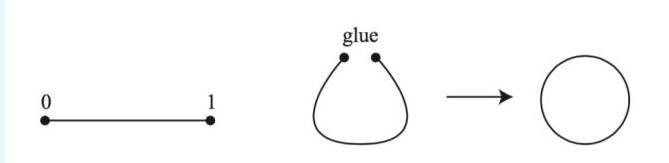
\includegraphics[max width=0.5\textwidth]{images/bo_d2bcsrref24c73avs720_67_642_1709_669_163_0.jpg}
\end{center}
\hspace*{3em} 

It is intuitive that the constructed quotient space should be homeomorphic to a circle \({S}^{1}\) . We will give a formal proof on this fact.

Proposition 6.3 Let \(X\) and \(Z\) be topological spaces, and \(\sim\) an equivalence relation on \(X\) .

Let \(g : X/ \sim   \rightarrow  Z\) be a function, and \(p : X \rightarrow  X/ \sim\) is a projection mapping The mapping \(g\) is continuous if and only if \(g \circ  p : X \rightarrow  Z\) is continuous.

Proof. 1. Necessity. Suppose that \(g\) is continuous. It’s clear that \(p\) is continuos, i.e, \(g \circ  p : X \rightarrow  Z\) is continuous.

2. Sufficiency. Suppose that \(g \circ  p : X \rightarrow  Z\) is continuous. Given any open \(U\) in \(Z\) , we imply \({\left( g \circ  p\right) }^{-1}\left( U\right)  = {p}^{-1}{g}^{-1}\left( U\right)\) is open in \(X\) . By definition of the quotient topology, we imply \({g}^{-1}\left( U\right)\) is open in \(X/ \sim\) . Therefore, \(g\) is continuous.

This useful lemma can be generalized into the case for generlized canonical projection mapping, called quotient mapping.

Definition 6.4 [Quotient mapping] A map \(p : X \rightarrow  Y\) between topological spaces is a quotient mapping if

1. \(p\) is surjective; and

2. \(p\) is continuous;

3. For any \(U \subseteq  Y\) such that \({p}^{-1}\left( U\right)\) is open in \(X\) , we imply \(U\) is open in \(Y\) .

The canonical projection map is clearly a quotient map. Actually, a stronger version of proposition (6.3) follows:

Proposition 6.4 Suppose that \(p : X \rightarrow  Y\) is a quotient map and that \(g : Y \rightarrow  Z\) is any mapping to another space \(Z\) . Then \(g\) is continuous iff \(g \circ  p\) is continuous.

Proof. The proof follows similarly as in proposition (6.3).

Now we give a formal proof of the conclusion in the example (6.5):

Proof. Define the mapping

\[
f : \;\left\lbrack  {0,1}\right\rbrack   \rightarrow  {S}^{1}
\]

\[
\text{ with }t \mapsto  \left( {\cos {2\pi t},\sin {2\pi t}}\right) \text{ . }
\]

Since \(f\left( 0\right)  = f\left( 1\right)\) , the function \(f\) induces a well-defined function

\[
g : \;\left\lbrack  {0,1}\right\rbrack  / \sim   \rightarrow  {S}^{1}
\]

\[
\text{ with }\left\lbrack  t\right\rbrack   \mapsto  f\left( t\right)
\]

such that \(f = g \circ  p\) , where \(p\) denotes the canonical projection mapping. Note that \(f\) is continuous. By proposition (6.3), we imply \(g\) is continuous. Furthermore,

1. Since \(\left\lbrack  {0,1}\right\rbrack\) is compact and \(p\) is continuous, we imply \(p\left( \left\lbrack  {0,1}\right\rbrack  \right)  = \left\lbrack  {0,1}\right\rbrack  / \sim\) is compact

2. \({S}^{1}\) is Hausdorff

3. \(g\) is a bijection

By applying theorem(5.3), we conclude that \(g\) is a homeomorphism, i.e., \(\left\lbrack  {0,1}\right\rbrack  / \sim\) and \({S}^{1}\) are homeomorphic.

The argument in the proof can be generalized into the proposition below:

Proposition 6.5 Let \(f : X \rightarrow  Y\) be a surjective continuous mapping between topologcial spaces. Let \(\sim\) be the equivalence relation on \(X\) defined by the partition \(\left\{  {{f}^{-1}\left( y\right)  \mid  y \in  Y}\right\}\) (i.e., \(f\left( x\right)  = \left( {x}^{\prime }\right)\) iff \(x \sim  {x}^{\prime }\) ). If \(X\) is compact and \(Y\) is Hausdorff, then \(X/ \sim\) and \(Y\) are homeomorphic.

\(\mathbb{R}\) The proposition (6.5) is a pattern of argument we should use several times. In order to show \(X/ \sim\) and \(Y\) are homeomorphic, we should think up a surjective continuous mapping \(f : X \rightarrow  Y\) "with respect to the identifications", i.e., \(f\left( {x}_{1}\right)  = f\left( {x}_{2}\right)\) whenever \({x}_{1} \sim  {x}_{2}\) . Therefore \(f\) will induce a well-defined function \(g : X/ \sim   \rightarrow  Y\) such that \(f = g \circ  f\) . Then checking the conditions in theorem(5.3) leads to the desired results.

Torus. We now study the torus in more detail.

1. Consider \(X = \left\lbrack  {0,1}\right\rbrack   \times  \left\lbrack  {0,1}\right\rbrack\) and define \(\left( {{s}_{1},{t}_{1}}\right)  \sim  \left( {{s}_{2},{t}_{2}}\right)\) if one of the following holds:

\begin{itemize}
\item \({s}_{1} = {s}_{2}\) and \({t}_{1} = {t}_{2}\) ;
\end{itemize}

\begin{itemize}
\item \(\left\{  {{s}_{1},{s}_{2}}\right\}   = \{ 0,1\} ,{t}_{1} = {t}_{2}\) ;
\end{itemize}

\begin{itemize}
\item \(\left\{  {{t}_{1},{t}_{2}}\right\}   = \{ 0,1\}\) and \({s}_{1} = {s}_{2}\) ;
\end{itemize}

\begin{itemize}
\item \(\left\{  {{s}_{1},{s}_{2}}\right\}   = \{ 0,1\} ,\left\{  {{t}_{1},{t}_{2}}\right\}   = \{ 0,1\}\)
\end{itemize}

The corresponding quotient space \(\left( {\left\lbrack  {0,1}\right\rbrack   \times  \left\lbrack  {0,1}\right\rbrack  }\right) / \sim\) is hoemomorhpic to the 2- dimension torus \({\mathbb{T}}^{2}\) .

Proof. Define the mapping \(f : \left\lbrack  {0,1}\right\rbrack   \times  \left\lbrack  {0,1}\right\rbrack   \rightarrow  {\mathbb{T}}^{2}\) as \(\left( {{t}_{1},{t}_{2}}\right)  \mapsto  \left( {{e}^{{2\pi i}{t}_{1}},{e}^{{2\pi i}{t}_{2}}}\right)\) .

(a) \(f\) is surjective, which also implies \({\mathbb{T}}^{2} = f\left( {\left\lbrack  {0,1}\right\rbrack   \times  \left\lbrack  {0,1}\right\rbrack  }\right)\) is compact.

(b) \({\mathbb{T}}^{2}\) is Hausdorff

(c) It’s clear that \(\left( {{s}_{1},{t}_{1}}\right)  \sim  \left( {{s}_{2},{t}_{2}}\right)\) implies \(f\left( {{s}_{1},{t}_{1}}\right)  = f\left( {{s}_{2},{t}_{2}}\right)\) . Conversely, suppose

\[
{e}^{{2\pi i}{s}_{1}} = {e}^{{2\pi i}{s}_{2}},\;{e}^{{2\pi i}{t}_{1}} = {e}^{{2\pi i}{t}_{2}}
\]

By the familiar property of \({e}^{ix}\) , we imply either \({t}_{1} = {t}_{2}\) or \(\left\{  {{t}_{1},{t}_{2}}\right\}   = \{ 0,1\}\) ; and

either \({s}_{1} = {s}_{2}\) or \(\left\{  {{s}_{1},{s}_{2}}\right\}   = \{ 0,1\}\)

By applying proposition (6.5), we conclude that \(\left( {\left\lbrack  {0,1}\right\rbrack   \times  \left\lbrack  {0,1}\right\rbrack  }\right) / \sim\) is homeomorphic to \({\mathbb{T}}^{2}\) .

2. Consider the closed disk \({\mathbb{D}}^{2} = \left\{  {\left( {x,y}\right)  \in  {\mathbb{R}}^{2} \mid  {x}^{2} + {y}^{2} \leq  1}\right\}\) , and defube \(\left( {{x}_{1},{y}_{1}}\right)  \sim  \left( {{x}_{2},{y}_{2}}\right)\) if one of the following holds:

\begin{itemize}
\item \({x}_{1} = {x}_{2}\) and \({y}_{1} = {y}_{2}\) ;
\end{itemize}

\begin{itemize}
\item \(\left( {{x}_{1},{y}_{1}}\right)\) and \(\left( {{x}_{2},{y}_{2}}\right)\) are in the boundary circle \({\mathbb{S}}^{1}\)
\end{itemize}

The corresponding quotient space \({\mathbb{D}}^{2}/ \sim\) is hoemomorhpic to the 2-dimension sphere \({\mathbb{S}}^{2} = \left\{  {\left( {x,y,z}\right)  \mid  {x}^{2} + {y}^{2} + {z}^{2} = 1}\right\}\) .

Proof. Define the mapping

\(f : \;{\mathbb{D}}^{2} \rightarrow  {\mathbb{S}}^{2}\)

with \(\left( {0,0}\right)  \mapsto  \left( {0,0,1}\right)\)

\[
\left( {x,y}\right)  \mapsto  \left( {\frac{x}{\sqrt{{x}^{2} + {y}^{2}}}\sin \left( {\pi \sqrt{{x}^{2} + {y}^{2}}}\right) ,\frac{y}{\sqrt{{x}^{2} + {y}^{2}}}\sin \left( {\pi \sqrt{{x}^{2} + {y}^{2}}}\right) ,\cos \left( {\pi \sqrt{{x}^{2} + {y}^{2}}}\right) }\right)
\]

It’s easy to check the conditions in proposition (6.5), and we conclude that \({\mathbb{D}}^{2}/ \sim\)

is hoemomorhpic to \({\mathbb{S}}^{2}\)

\section*{7.3. Monday for MAT4002}

\section*{7.3.1. Quotient Map}

Definition 7.6 [Quotient Map] A mapping \(q : X \rightarrow  Y\) between topological spaces is a quotient map if

1. \(q\) is surjective

2. For any \(U \subseteq  Y,U\) is open iff \({q}^{-1}\left( U\right)\) is open.

1. The canonical projection mapping \(p : X \rightarrow  X/ \sim\) is a quotient mapping

2. We say \(f\) is an open mapping if \(U\) is open in \(X\) implies \(f\left( U\right)\) is open in \(Y\) . Note that a continuous open mapping satisfies condition (2) in definition (7.6).

In proposition (6.5) we show the homeomorphism between \(X/ \sim\) and \(Y\) given the compactness of \(X\) and Hausdorffness of \(Y\) . Now we show the homeomorphism by replacing these conditions with the quotient mapping \(q\) :

Proposition 7.9 Suppose \(q : X \rightarrow  Y\) is a quotient map, and that \(\sim\) is an equivalence relation on \(X\) given by the partition \(\left\{  {{q}^{-1}\left( y\right)  \mid  y \in  Y}\right\}\) . Then \(X/ \sim\) and \(Y\) are homeomorphic.

Proof. Construct the mapping

\[
h : \;X/ \sim   \rightarrow  Y
\]

\[
\text{ with }h\left( \left\lbrack  x\right\rbrack  \right)  = q\left( x\right)
\]

Note that:

1. The mapping \(h\) is well-defined and injective.

2. Surjective is easy to shown.

3. The quotient mapping \(q \mathrel{\text{ := }} h \circ  p\) , by definition, is continuous. By applying proposition (6.4), \(h\) is continuous.

\begin{itemize}
\item For any open \(\widetilde{U} \subseteq  X/ \sim\) , it suffices to show \(h\left( \widetilde{U}\right)\) is open in \(Y\) .
\end{itemize}

Note that

\[
{q}^{-1}\left( {h\left( \widetilde{U}\right) }\right)  = {p}^{-1}{h}^{-1}\left( {h\left( \widetilde{U}\right) }\right)  = {p}^{-1}\left( \widetilde{U}\right) ,
\]

which is open by the definition of quotient topology (check proposition (6.1)).

Therefore, \(h\left( \widetilde{U}\right)\) is open by (2) in definition (7.6).

\begin{itemize}
\item Example 7.4 The \(\mathbb{R}/\mathbb{Z}\) is homeomorphic to the unit circle \({S}^{1}\) :
\end{itemize}

Define the mapping

\[
q : \mathbb{R} \rightarrow  {S}^{1}
\]

\[
x \mapsto  {e}^{2\pi ix}
\]

It's clear that

1. \(q\) is a continuous open mapping (why?)

2. \(q\) is surjective

Therefore, \(\mathbb{R}/ \sim   \cong  {S}^{1}\) , provided that \(x \sim  y\) iff \(q\left( x\right)  = q\left( y\right)\) , i.e., \(x - y \in  \mathbb{Z}\) . Therefore,

\[
\mathbb{R}/\mathbb{Z} \cong  {S}^{1}
\]

\section*{7.3.2. Simplicial Complex}

Combinatorics is the slums of topology. - J. H. C. Whitehead

The idea is to build some new spaces from some "fundamental" objects. The combina-torialists often study topology by the combinatorics of these fundamental objects. First we define what are the "fundamental" objects:

Definition 7.7 [ \(n\) -simplex] The standard \(n\) -simplex is the set

\[
{\Delta }^{n} = \left\{  {\left( {{x}_{1},\ldots ,{x}_{n + 1}}\right)  \in  {\mathbb{R}}^{n + 1} \mid  {x}_{i} \geq  0,\forall i\text{ and }\mathop{\sum }\limits_{{i = 1}}^{{n + 1}}{x}_{i} = 1}\right\}
\]

\begin{center}
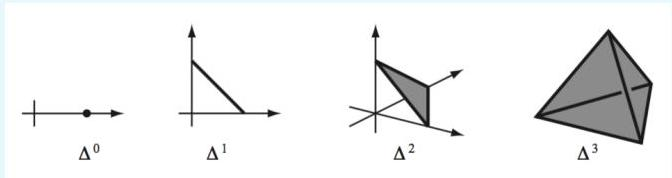
\includegraphics[max width=0.5\textwidth]{images/bo_d2bcsrref24c73avs720_73_642_599_672_178_0.jpg}
\end{center}
\hspace*{3em} 

Figure 7.1: Simplices on \({\mathbb{R}}^{2}\) are the triangles, so you may consider simplexes as the "triangles" in general spaces

1. The non-negative integer \(n\) is the dimension of this simplex

2. Its vertices, denoted as \(V\left( {\Delta }^{n}\right)\) , are those points \(\left( {{x}_{1},\ldots ,{x}_{n + 1}}\right)\) in \({\Delta }^{n}\) such that \({x}_{i} = 1\) for some \(i\) .

3. For each given non-empty \(\mathcal{A} \subseteq  \{ 1,\ldots ,n + 1\}\) , its face is defined as

\[
\left\{  {\left( {{x}_{1},\ldots ,{x}_{n + 1}}\right)  \in  {\Delta }^{n} \mid  {x}_{i} = 0,\forall i \notin  \mathcal{A}}\right\}
\]

In particular, \({\Delta }^{n}\) is a face of itself

4. The inside of \({\Delta }^{n}\) is

\[
\operatorname{inside}\left( {\Delta }^{n}\right)  \mathrel{\text{ := }} \left\{  {\left( {{x}_{1},\ldots ,{x}_{n + 1}}\right)  \in  {\Delta }^{n} \mid  {x}_{i} > 0,\forall i}\right\}
\]

In particular, the inside of \({\Delta }^{0}\) is \({\Delta }^{0}\) .

Definition 7.8 [Face Inclusion] A face inclusion of \({\Delta }^{m}\) into \({\Delta }^{n}\left( {m < n}\right)\) is a function \({\Delta }^{m} \rightarrow  {\Delta }^{n}\) which comes from the restriction of an injective linear map \(f : {\mathbb{R}}^{m + 1} \rightarrow  {\mathbb{R}}^{n + 1}\) that maps vertices in \({\Delta }^{m}\) into vertices in \({\Delta }^{n}\) .

For example, the linear transformation \(f : {\mathbb{R}}^{2} \rightarrow  {\mathbb{R}}^{3}\) defined below is a face inclusion:

\[
f\left( {1,0}\right)  = \left( {0,1,0}\right) ,\;f\left( {0,1}\right)  = \left( {0,0,1}\right) .
\]

R) Any injection mapping from \(\{ 1,\ldots ,m + 1\}  \rightarrow  \{ 1,\ldots ,n + 1\}\) gives a face inclusion \({\Delta }^{m} \rightarrow  {\Delta }^{n}\) , and vice versa.

Motivation. Now we build new spaces by making use of simplices. This new space is called the abstract complex. If a simplex is a part of the complex, so are all its faces.

Definition 7.9 [Abstract Simplicial Complex] An (abstract) simplicial complex is a pair \(K = \left( {V,\sum }\right)\) , where \(V\) is a set of vertices and \(\sum\) is a collection of non-empty finite subsets of

\(V\) (simplices) such that

1. For any \(v \in  V\) , the 1-element set \(\{ v\}\) is in \(\sum\)

2. If \(\sigma\) is an element of \(\sum\) , then so is any non-empty subset of \(\sigma\) .

For example, if \(V = \{ 1,2,3,4\}\) , then

\[
\sum  = \{ \{ 1\} ,\{ 2\} ,\{ 3\} ,\{ 4\} ,\{ 1,3,4\} ,\{ 2,4\} ,\{ 1,3\} ,\{ 3,4\} ,\{ 1,4\} \}
\]

We can associate to an abstract simplicial complex \(K\) a topological space \(\left| K\right|\) , which is called its geometric realization:

Definition 7.10 [Topological Realization] The topological realization of \(K = \left( {V,\sum }\right)\) is a topological space \(\left| K\right|\) (or denoted as \(\left| \left( {V,\sum }\right) \right|\) ), where

1. For each \(\sigma  \in  \sum\) with \(\left| \sigma \right|  = n + 1\) , take a copy of \(n\) -simplex and denote it as \({\Delta }_{\sigma }\)

2. Whenever \(\sigma  \subset  \tau  \in  \sum\) , identify \({\Delta }_{\sigma }\) with a face of \({\Delta }_{\tau }\) through face inclusion.

Or equivalently, \(\left| K\right|\) is a quotient space of the disjoint union

\[
\mathop{\coprod }\limits_{{\sigma  \in  \sum }}\sigma
\]

by the equivalence relation which identifies a point \(y \in  \sigma\) with its image under the face inclusion \(\sigma  \rightarrow  \tau\) , for any \(\sigma  \subset  \tau\) .

\begin{itemize}
\item Example 7.5 Take
\end{itemize}

\begin{center}
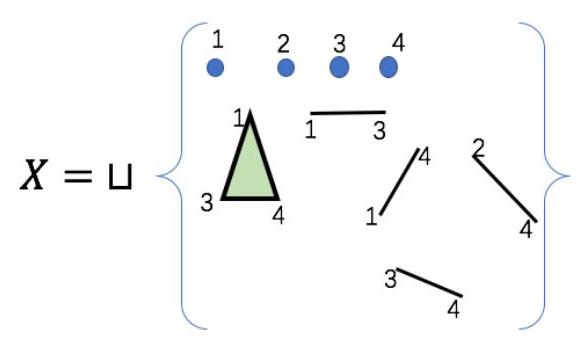
\includegraphics[max width=0.4\textwidth]{images/bo_d2bcsrref24c73avs720_75_692_801_582_343_0.jpg}
\end{center}
\hspace*{3em} 

As a result,

\begin{center}
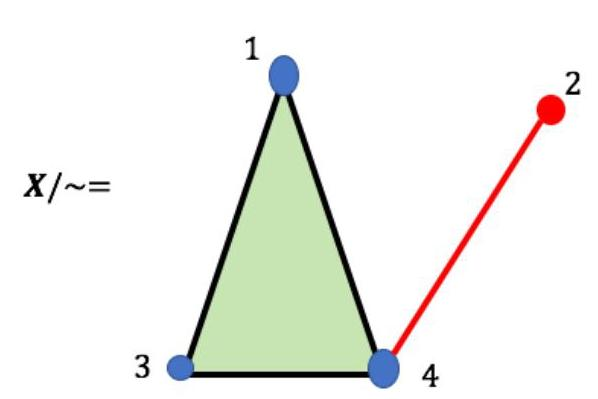
\includegraphics[max width=0.5\textwidth]{images/bo_d2bcsrref24c73avs720_75_669_1355_598_399_0.jpg}
\end{center}
\hspace*{3em} 

\begin{itemize}
\item Example 7.6 Take \(V = \{ 1,2,3,4\}\) and
\end{itemize}

\(\sum  = \{\) all subsets of \(V\) except \(V\}\)

As shown in the figure below, \(\left| \left( {V,\sum }\right) \right|  = {\Delta }^{3}\) :

\begin{center}
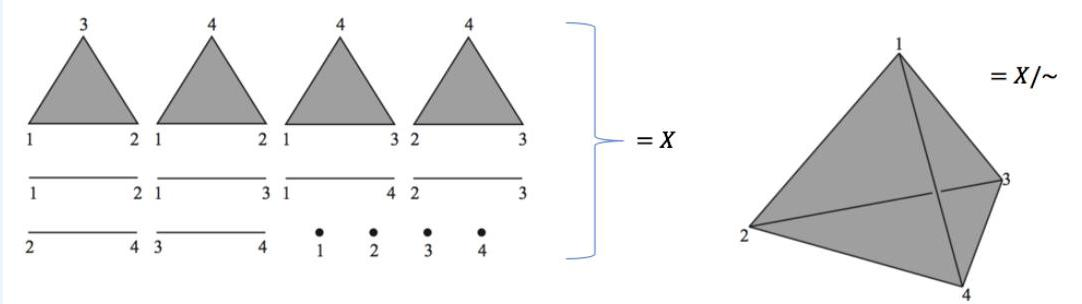
\includegraphics[max width=0.9\textwidth]{images/bo_d2bcsrref24c73avs720_76_274_640_1082_304_0.jpg}
\end{center}
\hspace*{3em} 

Definition 7.11 [Triangulation] A triangulation of a topological space \(X\) is a simplicial complex \(K = \left( {V,\sum }\right)\) together with a choice of homeomorphism \(\left| K\right|  \rightarrow  X\) .

\begin{itemize}
\item Example 7.7 The triangulation of \({S}^{1} \times  {S}^{1}\) can be realized by using nine vertices given below: (Try to identify \(X\) )
\end{itemize}

\begin{center}
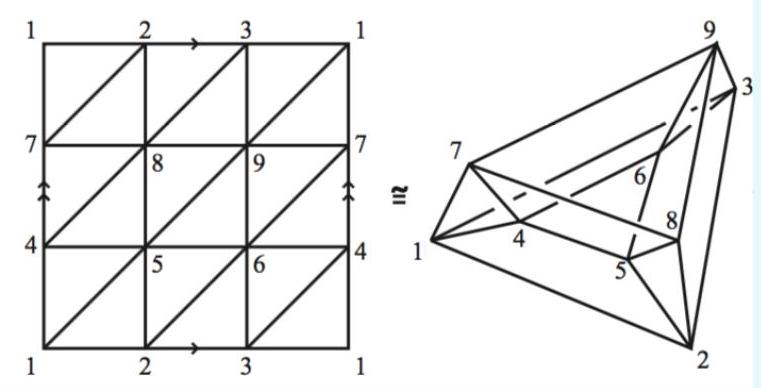
\includegraphics[max width=0.6\textwidth]{images/bo_d2bcsrref24c73avs720_76_468_1487_761_388_0.jpg}
\end{center}
\hspace*{3em} 

Figure 7.2: The quotient space \(\left| K\right|  \mathrel{\text{ := }} X/ \sim\)

\section*{7.5. Wednesday for MAT4002}

\section*{7.5.1. Remarks on Triangulation}

Consider the simplical complex \(K = \left( {V,\sum }\right)\) with

\[
V = \{ 1,2,3,4,\ldots ,9\} ,\;\sum  = \left\{  \begin{array}{r} 9\text{ subsets with }1\text{ element } \\  {27}\text{ subsets with }2\text{ elements } \\  {18}\text{ subsets with }3\text{ elements } \end{array}\right.
\]

We start to build the topological realization of \(K\) with 90-simplicies,271-simplicies, and 18 2-simplicies. The identification of them is as follows:

\begin{center}
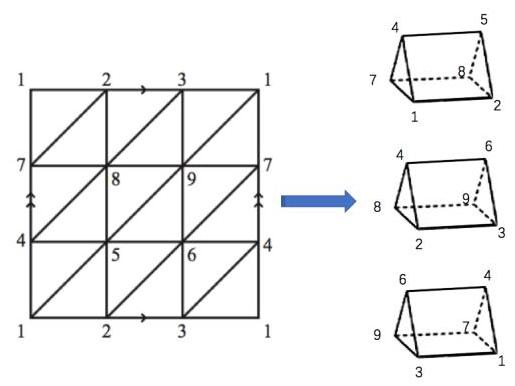
\includegraphics[max width=0.4\textwidth]{images/bo_d2bcsrref24c73avs720_77_543_985_515_386_0.jpg}
\end{center}
\hspace*{3em} 

Figure 7.3: Step 1: Identify 3 columns separately, i.e., identify \(\{ 1,7,4,1,2,8,5,2\}\) , \(\{ 2,8,5,2,3,9,6,3\}\) , and \(\{ 3,9,6,3,1,7,4,1\}\) .

\begin{center}
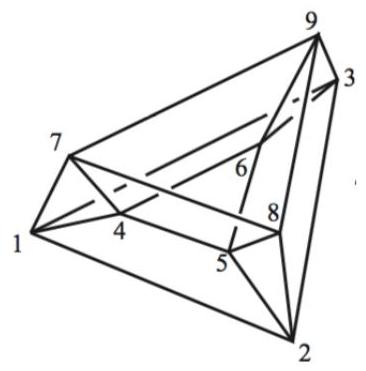
\includegraphics[max width=0.3\textwidth]{images/bo_d2bcsrref24c73avs720_77_643_1563_366_371_0.jpg}
\end{center}
\hspace*{3em} 

Figure 7.4: Step 2: "gluing" these three prisms in the figure above together.

Question: why \(K\) is homeomorphic to the torus?

\begin{center}
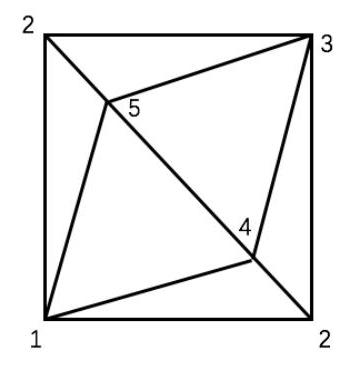
\includegraphics[max width=0.2\textwidth]{images/bo_d2bcsrref24c73avs720_78_787_416_344_369_0.jpg}
\end{center}
\hspace*{3em} 

The \(\left| \left( {V,\sum }\right) \right|\) is homeomorphism to the quotient space \({S}^{1}\) plotted below

\begin{center}
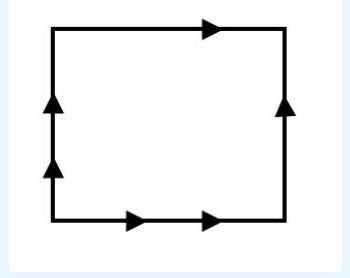
\includegraphics[max width=0.2\textwidth]{images/bo_d2bcsrref24c73avs720_78_805_984_350_278_0.jpg}
\end{center}
\hspace*{3em} 

Furthermore, can we build a triangulation of the tours using fewer simplices? The answer is no. Consider the figure below: at the bottom edge of this square, there are two 1-simplicies lablled \(\{ 1,2\}\) , which cannot happen in a tours.

\begin{center}
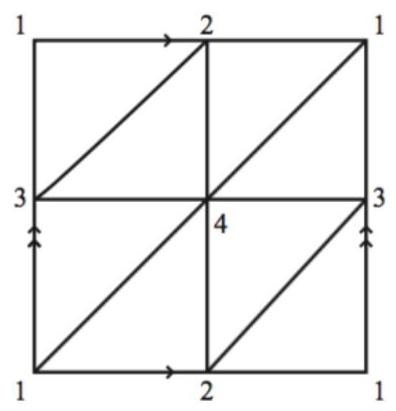
\includegraphics[max width=0.3\textwidth]{images/bo_d2bcsrref24c73avs720_78_773_1700_396_411_0.jpg}
\end{center}
\hspace*{3em} 

\begin{center}
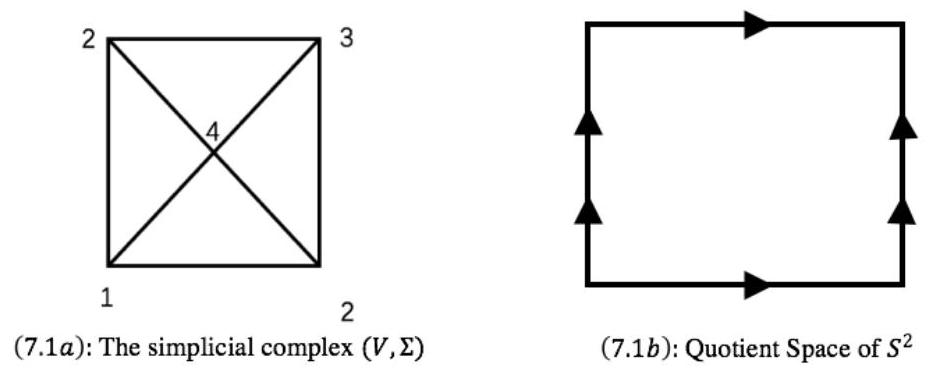
\includegraphics[max width=0.7\textwidth]{images/bo_d2bcsrref24c73avs720_79_347_434_929_377_0.jpg}
\end{center}
\hspace*{3em} 

Answer: No. Since the 2-simplex \({\Delta }_{\{ 2,3,4\} }\) appears twice in the Fig. (7.1a), the tri-angluation of this figure means that we need to stick the top triangle and the right triangle together, which contradicts to the structure of the quotient space \({S}^{2}\) shown in Fig. (7.1b).

The simplicial complex gives us another way to study \(X\) , i.e., it suffices to study \(\left( {V,\sum }\right)\) such that \(\left| \left( {V,\sum }\right) \right|  \cong  X\) . The question is that can we distinguish \(X = {S}^{1} \times  {S}^{1}\) and \(Y = {S}^{2}\) ? In other words, can we distinguish the difference of corresponding topological realizations?

Theorem 7.2 - Euler’s Formula. Suppose that \(\left| \left( {{V}_{1},{\sum }_{1}}\right) \right|  \cong  \left| \left( {{V}_{2},{\sum }_{2}}\right) \right|\) , then

\[
\mathop{\sum }\limits_{{i = 1}}^{\infty }{\left( -1\right) }^{i}\text{ (number of subsets in }{\sum }_{1}\text{ with }\left( {i + 1}\right) \text{ -element) }
\]

\[
= \mathop{\sum }\limits_{{i = 1}}^{\infty }{\left( -1\right) }^{i}\text{ (number of subsets in }{\sum }_{2}\text{ with }\left( {i + 1}\right) \text{ -element) }
\]

From previous examples we can see that \(\mathcal{X}\left( {S}^{2}\right)  = 5 - 9 + 6 = 2\) and \(\mathcal{X}\left( {{S}^{1} \times  {S}^{1}}\right)  =\)  \(9 - {27} + {18} = 0\) , which implies

\[
{S}^{2} ≆ {S}^{1} \times  {S}^{1}
\]

\section*{7.5.2. Simplicial Subcomplex}

Definition 7.13 [Simplicial Subcomplex] A subcomplex of a simplicial complex \(K = \left( {V,\sum }\right)\) is a simplicial complex \({K}^{\prime } = \left( {{V}^{\prime },{\sum }^{\prime }}\right)\) such that

\[
{V}^{\prime } \subseteq  V,\;{\sum }^{\prime } \subseteq  \sum
\]

Proposition 7.13 Suppose \({K}^{\prime }\) is subcomplex of \(K\) , then \(\left| {K}^{\prime }\right|\) is closed in \(\left| K\right|\) .

Proof. Suppose that \(D\) is the disjoint union of all the simplicial complex forming \(\left| K\right|\) . (note that the number of component in \(D\) is \(\left| \sum \right|\) )

Consider the canonical projection mapping \(D \rightarrow  \left| K\right|\) . Observe that \({p}^{-1}\left( \left| {K}^{\prime }\right| \right)\) precisely equals to \(\mathop{\coprod }\limits_{{{\sigma }^{\prime } \in  {\sum }^{\prime }}}{\sigma }^{\prime }\) , which is closed in \(D\) . By definition of quotient topology, \(\left| {K}^{\prime }\right|\) is also closed.

Definition 7.14 [Subcomplex spanned by vertices] Let \(K = \left( {V,\sum }\right)\) be a simplicial complex and \({V}^{\prime } \subseteq  V\) . Then the subcomplex spanned by \({V}^{\prime }\) is \(\left( {{V}^{\prime },{\sum }^{\prime }}\right)\) such that

\begin{itemize}
\item \({V}^{\prime }\) denotes the vertex set.
\end{itemize}

\begin{itemize}
\item the simplices \({\sum }^{\prime }\) is given by
\end{itemize}

\[
\left\{  {\sigma  \in  \sum  \mid  \sigma  \subseteq  {V}^{\prime }}\right\}
\]

Definition 7.15 [Link and Star] Let \(\left( {V,\sum }\right)  = K\) be simplicial complex

\begin{itemize}
\item The link of \(v \in  V\) , denoted as \(\operatorname{lk}\left( v\right)\) is the sub-complex with
\end{itemize}

\begin{itemize}
\item vertex set
\end{itemize}

\[
\{ w \in  V \smallsetminus  \{ v\}  \mid  \{ v,w\}  \in  \sum \}
\]

\begin{itemize}
\item simplicies
\end{itemize}

\[
\{ \sigma  \in  \sum  \mid  \mathbf{v} \notin  \sigma \text{ and }\sigma  \cup  \{ \mathbf{v}\}  \in  \sum \}
\]

\begin{itemize}
\item The star of \(v\) (denoted as \(\operatorname{st}\left( v\right)\) ) is
\end{itemize}

\[
\bigcup \{ \operatorname{inside}\left( \sigma \right)  \mid  \sigma  \in  \sum ,v \in  \sigma \}
\]

Proposition \({7.14}\;\mathrm{{st}}\left( v\right)\) is open and \(v \in  \mathrm{{st}}\left( v\right)\) .

Proof. Omitted.

In fact, \(\left| K\right|  \smallsetminus  \operatorname{st}\left( v\right)\) is the simplicial subcomplex spanned by \(V\) .

\section*{7.5.3. Some properties of simplicial complex}

Proposition 7.15 Suppose that \(K = \left( {V,\sum }\right)\) , where \(V\) is finite. Then \(\left| K\right|\) is compact.

Proof. The mapping \(p : D \rightarrow  \left| K\right|\) is a canonical projection mapping, which is continuous; and \(D\) (the finite disjoint union of \({\Delta }_{\sigma }\) ’s) is compact.

Therefore, \(p\left( D\right)  = \left| K\right|\) is compact.

Proposition 7.16 For any simplicial complex \(K = \left( {V,\sum }\right)\) , where \(V\) is finite, there is a continuous injection

\[
f : \left| K\right|  \rightarrow  {\mathbb{R}}^{n}\text{ for some }n
\]

Proof. Let \({K}^{\prime } = \left( {V,{\sum }^{\prime }}\right)\) , where \({\sum }^{\prime } =\) power set of \(V\) . Then

\[
\left| {K}^{\prime }\right|  = {\Delta }^{\left| V\right|  - 1} \subseteq  {\mathbb{R}}^{\left| V\right| }
\]

Consider the inclusion

\[
i : \left| K\right|  \rightarrow  \left| {K}^{\prime }\right|
\]

which comes from the following:

1. Consider the \(D \mathrel{\text{ := }} \mathop{\coprod }\limits_{{\sigma  \in  \sum }}{\Delta }_{\sigma }\) and \({D}^{\prime } = \mathop{\coprod }\limits_{{{\sigma }^{\prime } \in  {\sum }^{\prime }}}{\Delta }_{{\sigma }^{\prime }}\) in \(\left( {V,\sum }\right)\) and \(\left( {V,{\sum }^{\prime }}\right)\)

2. Construct the mapping \(\widetilde{i} : D \hookrightarrow  {D}^{\prime }\overset{{p}^{\prime }}{ \rightarrow  }\left| K\right|\) .

3. The mapping \(\widetilde{i}\) descends to \(i : D/ \sim   \rightarrow  \left| {K}^{\prime }\right|\) (try to write down the detailed mapping), which is continuous and injective.

Therefore, \(\left| K\right|  \hookrightarrow  \left| {K}^{\prime }\right|\) , i.e., \(\left| K\right|  \hookrightarrow  {\mathbb{R}}^{n}\) . The proof is complete.

\section*{8.5. Wednesday for MAT4002}

Reviewing. We can construct a continuous injection from \(\left| K\right|\) to \(\left| {K}^{\prime }\right|\) , where \(K = \left( {V,\sum }\right)\) is a simplicial complex, and \({K}^{\prime } = \left( {{V}^{\prime },{\sum }^{\prime }}\right)\) is its subcomplex:

Let \({D}_{\sum } \mathrel{\text{ := }} \mathop{\coprod }\limits_{{\sigma  \in  \sum }}\sigma\) and \({D}_{{\sum }^{\prime }} \mathrel{\text{ := }} \mathop{\coprod }\limits_{{{\sigma }^{\prime } \in  {\sum }^{\prime }}}{\sigma }^{\prime }\) , then \(\left| {K}^{\prime }\right|  = {D}_{{\sum }^{\prime }}/{ \sim  }_{{\sum }^{\prime }}\) and \(\left| K\right|  = {D}_{\sum }/{ \sim  }_{\sum }\) , which

follows that

\(f : {D}_{{\sum }^{\prime }} \rightarrow  {D}_{\sum }\overset{P}{ \rightarrow  }{D}_{\sum }/{ \sim  }_{\sum },\;P\) denotes the canonical projection mapping

The whole mapping \(f\) descends to a continuous mapping

\[
\widetilde{f} : {D}_{{\sum }^{\prime }}/{ \sim  }_{{\sum }^{\prime }} \rightarrow  {D}_{\sum }/{ \sim  }_{\sum }
\]

The \(\widetilde{f}\) is injective since

\[
x{ \sim  }_{{\sum }^{\prime }}y \Leftrightarrow  i\left( x\right) { \sim  }_{\sum }i\left( y\right) ,\;\forall x,y \in  {D}_{\sum }, \tag{8.14}
\]

where \(i\) denotes the inclusion mapping.

Another way is to consider the inclusion \(i : \left| {K}^{\prime }\right|  \rightarrow  \left| K\right|\) , which is continuous and injective as well. Note that \(i\left( \left| {K}^{\prime }\right| \right)\) is closed in \(\left| K\right|\) .

Proposition 8.7 For each \(K = \left( {V,\sum }\right)\) , and finite \(V\) , there is a continuous injection \(g : \left| K\right|  \hookrightarrow  {\mathbb{R}}^{n}\) for some \(n\) .

Proof. Consider \({K}^{p} \mathrel{\text{ := }} \left( {V,{\sum }^{p}}\right)\) , where \({\sum }^{p}\) is the power set of \(V\) . Therefore, \(\left| {K}^{p}\right|  = {\Delta }^{\left| V\right|  - 1} \subseteq\)  \({\mathbb{R}}^{\left| V\right| }\) , and \(K\) is a simplicial subcomplex of \({K}^{p}\) , which follows that

\[
l : \left| {K}^{\prime }\right| \overset{i}{ \rightarrow  }\left| {K}^{p}\right| \overset{i}{ \rightarrow  }{\mathbb{R}}^{\left| V\right| }
\]

The whole mapping \(l\) is an inclusion mapping from \(\left| {K}^{\prime }\right|\) to \({\mathbb{R}}^{\left| V\right| }\) , which is continuous and injective. The proof is complete.

Proposition 8.8 - Hausdorff. If \(K = \left( {V,\sum }\right)\) with fintie \(V\) , then \(\left| K\right|\) is Hausdorff.

Proof. Let \(g : \left| K\right| \overset{l}{ \rightarrow  }{\mathbb{R}}^{n}\) . Consider the bijective \(g : \left| K\right|  \rightarrow  g\left( \left| K\right| \right)\) , which is continuous.

Sicne \(\left| K\right|\) is compact, and \(g\left( \left| K\right| \right)  \subseteq  {\mathbb{R}}^{n}\) is Hausdorff, we imply that \(\left| K\right|\) and \(g\left( \left| K\right| \right)\) are homeomorphic, i.e., \(\left| K\right|\) is Hausdorff.

Definition 8.14 [Edge Path] An edge path of \(K = \left( {V,\sum }\right)\) is a sequence of vertices \(\left( {{v}_{1},\ldots ,{v}_{n}}\right) ,{v}_{i} \in  V\) such that \(\left\{  {{v}_{i},{v}_{i + 1}}\right\}   \in  \sum ,\forall i\) .

Proposition 8.9 - Connectedness. Let \(K = \left( {V,\sum }\right)\) be a simplicial complex. TFAE:

1. \(\left| K\right|\) is connected

2. \(\left| K\right|\) is path-connected

3. Any 2 vertices in \(\left( {V,\sum }\right)\) can be joined by an edge path, i.e., for \(\forall u,v \in  V\) , there exists \({v}_{1},\ldots ,{v}_{k} \in  V\) such that \(\left( {u,{v}_{1},\ldots ,{v}_{k},v}\right)\) is an edge path.

Sketch of Proof (to be revised). 1. (3) implies (2): For every \(x,y \in  \left| K\right|\) ,

\[
\left\{  \begin{array}{l} x \in  {\Delta }_{{\sigma }_{1}}\text{ for some }{\sigma }_{1} \in  \sum . \\  y \in  {\Delta }_{{\sigma }_{2}}\text{ for some }{\sigma }_{2} \in  \sum . \end{array}\right.
\]

Take a path joining \(x\) to a vertex \({v}_{1} \in  {\sigma }_{1}\) and a path joining \(y\) to a vertex \({v}_{2} \in  {\sigma }_{2}\) . By (3), we have a path joninig \({v}_{1}\) and \({v}_{2}\) .

2. (1) implies (3): Suppose on the contrary that there is a vertex \(v\) not satisfying (3). Take \({V}^{\prime }\) as the set of vertexs that can be joined with \(v\) ; and \({V}^{\prime \prime }\) as the set of vertexs that cannot be joinied with \(v\) .

Then \({V}^{\prime },{V}^{\prime \prime } \neq  \varnothing\) . Consider \({K}^{\prime },{K}^{\prime \prime }\) be simplicial subcomplexes of \(K\) , spanned by \({V}^{\prime }\) and \({V}^{\prime \prime }\) . Then \(\left| {K}^{\prime }\right| ,\left| {K}^{\prime \prime }\right|\) are disjoint, closed in \(\left| K\right|\) .

\(\left| K\right|  = \left| {K}^{\prime }\right|  \cup  \left| {K}^{\prime \prime }\right|\) . If there exists \(x \in  \left| K\right|  \smallsetminus  \left( {\left| {K}^{\prime }\right|  \cup  \left| {K}^{\prime \prime }\right| }\right)\) , then for any \(\sigma  \in  \sum\) such that \(x \in  {\Delta }_{\sigma }\) , we imply \({\Delta }_{\sigma } \nsubseteq  \left| {K}^{\prime }\right|\) or \(\left| {K}^{\prime \prime }\right|\) .

Therefore, \(\sigma\) consists of vertices in both \({V}^{\prime }\) and \({V}^{\prime \prime }\) . Then there is \({v}^{\prime },{v}^{\prime \prime } \in  \sigma\) joining \({V}^{\prime }\) and \({V}^{\prime \prime }\) .

Therefore, there is no such \(x\) and hence \(\left| K\right|  = \left| {K}^{\prime }\right|  \cup  \left| {K}^{\prime \prime }\right|\) is a disjoint union of two closed sets, i.e., not connected.